\section{Autómatas o Máquinas de Estado}

Existen muchas formas de modelar el comportamiento de los sistemas, y el uso de
máquinas de estado finitas es una de las más antiguas y más conocidas.
Las máquinas de estado finitas o autómatas nos permiten pensar acerca del
``estado'' de un sistema en un instante en particular y caracterizar el comportamiento de dicho
sistema basado en ese estado. El uso de esta técnica de modelado no está
limitada al desarrollo de sistemas de software.\cite{FSM_Wright}

\subsection{Definición Conceptual de Máquina de Estado}

Si una máquina de estados M, en un instante dado, se encuentra en el estado
$E_{0}$ y ocurre un evento $e_{0}$ que lleva a M al estado $E_{1}$, se
dice que ocurrió una \textit{transición} del estado $E_{0}$ al estado
$E_{1}$.
A partir de esto se puede deducir que M no puede estar en $E_{0}$ y $E_{1}$
a la vez, y por lo tanto los estados de una máquina de estados, son
\textbf{estados globales} del sistema modelado.

Analizando la semántica de las máquinas de estado, se pueden
identificar algunas características clave de un sistema que puede ser modelado con máquinas de
estados finitas:
\begin{itemize}
  \item El sistema debe ser descripto por conjunto finito de estados.
  \item El sistema debe tener una cantidad finita de entradas y/o eventos que
  puedan disparar transiciones entre estados.
  \item El comportamiento del sistema en un instante dado depende del estado
  actual y de sus entradas o eventos que ocurran en ese instante.
  \item Para cada estado posible en que el sistema pueda encontrarse existe un
  comportamiento definido para cada posible entrada o evento.
  \item El sistema tiene un estado inicial único y definido.
\end{itemize} \cite{FSM_Wright}

\subsection{Definición Formal de Máquina de Estado}

A fin de eliminar la ambigüedad existente en una definición conceptual, se
introduce una definición formal de Autómata Finito:
\newline\newline\emph{Definición:} Un autómata finito M está definido por una
tupla $(\Sigma, Q, q_{0}, F, \sigma)$, donde:
\begin{itemize}    
  \item $\Sigma$ es el conjunto de símbolos de entrada de M
  \item $Q$ es el conjunto de estados de M
  \item $q_{0}$ es el estado inicial de M
  \item $F \subseteq Q$ es el conjunto de estados finales de M
  \item $\sigma : Q  \times \Sigma \rightarrow Q$ es la función de
  transición
\end{itemize} \cite{FSM_Wright}

\section{Redes de Petri}
\label{redes_de_petri}

Tomando el concepto de transición en una máquina de estados, se lo puede
extender a una entidad propia.
Esta transitión $t_{i}$ será denotada por una barra, un rectángulo o un
cuadrado, y puede tener múltiples arcos de entrada (entrantes) y de salida
(salientes) a la vez. Esta transición, representa la \textit{transición} básica
de una Red de Petri (RdP).\cite{PetriNetsFundamentals}

De la misma forma que en una máquina de estados los círculos denotan estados
del sistema, en una RdP se utilizan círculos para denotar las \textit{plazas} o
\textit{lugares} de la red. Estas plazas no representan estados globales, sino
\textbf{estados locales}. \cite{PetriNetsFundamentals} El estado de una plaza
está dado por la cantidad de marcas o \textit{tokens} que esta contiene.

Las \textit{plazas} y las \textit{transiciones} de una RdP se conectan entre sí
mediante \textit{arcos} dirigidos, pudiéndose unir una plaza únicamente con cero
o más transiciones y viceversa. La unión entre plazas o entre transiciones no
respeta la estructura del modelo.

Como consecuencia de esto, una RdP puede ser representada por un grafo
bipartito, donde los nodos pertenecen a uno de dos conjuntos (\textit{plazas} o
\textit{transiciones}).

\begin{figure}[h]
	\centering
	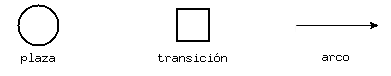
\includegraphics[width=75mm]{Partes_De_Una_Red}
	\caption{Partes de una Red de Petri}
	\label{fig:partes_de_una_red}
\end{figure}

Se pueden visualizar las partes de una Red de Petri en la figura
\ref{fig:partes_de_una_red}.\\

\begin{figure}[h]
    \centering
    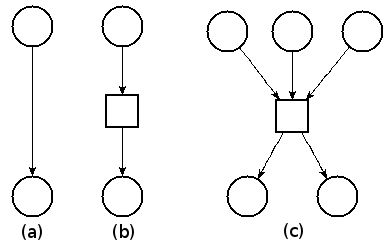
\includegraphics[height=40mm]{Automata_Y_Petri}
    \caption{Equivalencia entre una Máquina de Estados y una Red de Petri}
    \label{fig:automata_y_petri}
\end{figure}

En la figura \ref{fig:automata_y_petri} se aprecia:\\
\begin{itemize}
  \item[(a)] Una máquina de estados de dos estados y una transición.
  \item[(b)] Una RdP equivalente a la máquina de (a).
  \item[(c)] Una RdP con una transición con múltiples arcos de entrada y de
  salida.
\end{itemize}

Se puede extraer como consecuencia directa de esta extensión de la semántica de
un autómata que en una Red de Petri:
\begin{itemize}
  \item Múltiples tokens pueden existir en el modelo al mismo tiempo, y
  particularmente en una plaza.
  \item No existe un estado global explícito.
  \item El estado global del sistema es el conjunto de todos los estados
  parciales, representados por las plazas y sus tokens. A este conjunto se lo
  denomina el \textbf{marcado} de la red.
\end{itemize}

\subsection{Definición Formal de Red de Petri}
\label{def_formal_petri}
A fin de eliminar ambigüedades, se presenta una serie de definiciones sobre
Redes de Petri.

\begin{itemize}
  \stepcounter{definitionsCounter}
  \item [\underline{Definición \thedefinitionsCounter}:] Una Red de Petri R está
  definida por la tupla $(P, T, Pre, Post)$ donde:
  \begin{itemize}
    \item $ P = \{ p_1, p_2, \ldots, p_p \} $ un conjunto de plazas.\footnote{Se
    utiliza $p$ como la cantidad de plazas de la RdP en todo momento dentro de este informe por simplicidad para el lector}
    \item $ T = \{ t_1, t_2, \ldots, t_t \} $ un conjunto de transiciones, donde
    $ P \cap T = \emptyset $. \footnote{Se utiliza $t$ como la cantidad de
    transiciones de la RdP en todo momento dentro de este informe por
    simplicidad para el lector}
    \item $ Pre: P \times T \rightarrow \mathbb{N}^{p} $ aplicación de
    precedencia.\footnote{Se toma la definición de números naturales incluyendo
    el cero por simplicidad de notación.}
    \item $ Post: P \times T \rightarrow \mathbb{N}^{p} $ aplicación de
    incidencia.
  \end{itemize}
  $ Pre (p_i, t_j) $ contiene el peso del arco que va de $ p_i $ a $ t_j $, y
  $ Post (p_i, t_j) $ contiene el peso del arco que va de $ t_j $ a $ p_i $

  \stepcounter{definitionsCounter}
  \item [\underline{Definición \thedefinitionsCounter}:] Una Red de Petri Marcada está
  definida por el par $(R, M)$, donde R es una RdP y $ M : P \rightarrow
  \mathbb{N}^{p}$ (donde $\left\vert{P}\right\vert = p $) es una aplicación
  llamada \textit{marcado}.\\
  $m(R)$, o más simplemente $m$ si la red es conocida, define el marcado de la
  RdP y $m(p_{i})$ o $m_{p_{i}}$ indica el marcado de la plaza $p_{i}$, es
  decir, el número de tokens contenido en la plaza $p_{i}$.\\
  La marca inicial se denota $m_{0}$ y da la cantidad inicial de tokens en todas
  las plazas de la red, por lo que especifica el estado inicial del sistema.
  
  \stepcounter{definitionsCounter}
  \item [\underline{Definición \thedefinitionsCounter}:] Para una marca $m$, una transición $t_{j}$
  está sensibilizada, y por lo tanto es disparable, si y solo si:\\
  $$ \forall p_{i} \in P, m(p_i) \geq Pre(p_{i}, t_{j}) $$
  Conceptualmente, una transición está sensibilizada si todas sus plazas de
  entrada contienen al menos la cantidad de tokens que indica el peso de los
  arcos que las unen.

  En la figura \ref{fig:transiciones_no_sensibilizadas} se observa gráficamente esta definición mediante dos casos de transiciones no sensibilizadas. Nótese
  el peso de los arcos.

  \begin{figure}[h]
    \centering
    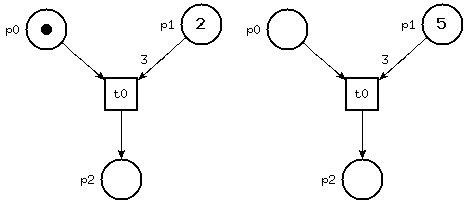
\includegraphics[height=40mm]{Transiciones_No_Sensibilizadas}
    \caption{Ejemplos de transiciones no sensibilizadas.}
    \label{fig:transiciones_no_sensibilizadas}
  \end{figure}
  
  \stepcounter{definitionsCounter}
  \item [\underline{Definición \thedefinitionsCounter}:] La estructura de una Red de Petri
  se denota $ N = \{P, T, F, W\} $ donde,
  \begin{itemize}
    \item $P$ es en conjunto de plazas.
    \item $T$ es el conjunto de transiciones, donde se cumple que $ P \cap T =
    \emptyset $
    \item $F$ es el conjunto de arcos, donde $ F \subseteq (P
    \times T) \cup (F \times P) $.
    \item $W$ es la función de peso de los arcos.
  \end{itemize}

  \stepcounter{definitionsCounter}
  \item [\underline{Definición \thedefinitionsCounter}:] Conjunto de transición y plaza de entrada y
  de salida.
  \begin{itemize}
    \item[] El conjunto de las plazas de entrada a la transición $t$ se denota
    $\bullet t$ y se define,
    $$ \bullet t = \{ p \in P : (p, t) \in F \} $$
    \item[] El conjunto de las plazas de salida de la transición $t$ se denota $
    t \bullet$ y se define,
    $$ t \bullet = \{ p \in P : (t, p) \in F \} $$
    \item[] El conjunto de las transiciones de entrada a la plaza $p$ se
    denota $\bullet p$ y se define,
    $$ \bullet p = \{ t \in T : (t, p) \in F \} $$
    \item[] El conjunto de las transiciones de salida de la plaza $p$ se denota
    $ p \bullet$ y se define,
    $$ p \bullet = \{ t \in T : (p, t) \in F \} $$
  \end{itemize}
\end{itemize}

\subsection{Disparo de una Transición}

La condición de disparo relacionada a $Pre(p_{i}, t_{j})$ significa que para
todas las plazas $p_{i}$ de entrada a $t_{j}$, es decir, todas las plazas que
tienen arcos que apuntan hacia $t_{j}$, el número de tokens presentes debe ser
mayor o igual al peso de dicho arco.

\begin{itemize}
  \stepcounter{definitionsCounter}
  \item [\underline{Definición \thedefinitionsCounter}:] En una RdP, dada una marca $ m_{n}(p) $,
  cualquier transición $ t_{j} $ que se encuentre sensibilizada puede ser
  disparada, y su disparo lleva a una marca $ m_{n+1}(p)$ dada por:
  $$ m_{n+1}(p) = m_{n}(p) + Post(p_{i}, t_{j}) - Pre(p_{i}, t_{j}), \forall
  p_{i} \in P $$
  Como se indica en la ecuación, al disparar la transición $ t_{j} $, se quitan
  tantos tokens de $ \bullet t $ como indiquen los arcos que las unen a $ t_{j}
  $, y se añaden a $ t \bullet $ la cantidad de tokens que indiquen los arcos
  que unen a $ t_{j} $ con ellas.\\
  El disparo de una transición $ t_{j} $ se denota $ m_{n}\rightarrow t_{j}
  \rightarrow m_{n+1} $

  En la figura {\ref{fig:disparo_transicion}} se observa el estado de una RdP
  antes y después del disparo de una transición.
  \begin{figure}[h]
    \centering
    \subfigure[$t_{0}$ sensibilizada]{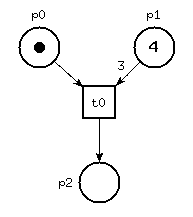
\includegraphics[height=40mm]{Red_Sensibilizada}}
    \subfigure[Disparo de $t_{0}$]{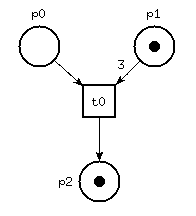
\includegraphics[height=40mm]{Red_Disparada}}
    \caption{Disparo de una transición}
    \label{fig:disparo_transicion}
  \end{figure}
  
  \stepcounter{definitionsCounter}
  \item [\underline{Definición \thedefinitionsCounter}:] Matriz de Incidencia.\\
  La matriz de incidencia de una RdP se define como,
  $$ I = Post - Pre $$
  \textbf{Notas:}
  \begin{itemize}
    \item El disparo de una transición $t_{j}$ se reformula como, $$ m_{n+1}(p)
    = m_{n}(p) + I(p_{i}, t_{j}), \forall p_{i} \in P $$
    \item A partir de las matrices $Pre$ y $Post$ se puede reconstruir la
    estructura de la red, a partir de $I$ no es posible.
  \end{itemize}
\end{itemize}

\subsection{Sucesión de Disparos}

Si en lugar del disparo de una transición se requiere disparar múltiples
transiciones, se puede reescribir la ecuación de cambio de estado de la red de
la siguiente forma,
$$ m_{n+1} = m_{n} + I \times \sigma $$
En esta ecuación, $\sigma$ representa la sucesión de disparos a realizar. Se
cumple $\sigma \in \mathbb{N}^{t}$ y el elemento $\sigma_{i}$ contiene la
cantidad de disparos a realizar sobre $t_{i}$.\\
Si se comienza a realizar la sucesión de disparos $\sigma_{i}$ a partir del
marcado inicial $m_{0}$ y todos los disparos son exitosos, se llega a un marcado
$m_{i}$ y se dice que $m_{i}$ es \textit{alcanzable}.\\
De la misma forma, si existe un marcado $m_{j}$ alcanzable desde $m_{0}$, debe
exitir una sucesión de disparos $\sigma_{j}$ que permita alcanzarlo.

\section{Extensión de la Semántica de las Redes de Petri}

Las RdP descriptas anteriormente constituyen la versión más simple de este
modelo, conocidas como \textit{Redes de Petri Plaza-Transición} o \textit{Redes
de Petri Ordinarias}.

Se pueden realizar modificaciones sobre el modelo a fin de aumentar la semántica
y permitir modelar mayor cantidad de sistemas del mundo real.

Algunas de las variantes introducidas a las RdP desde su aparición son:
\begin{itemize}
  \item Semántica Temporal: Permiten modelar restricciones temporales sobre la
  acciones.
  \item Semántica Estocástica: Permiten modelar restricciones ligadas a 
  variables aleatorias.
  \item Arcos Especiales: Tienen alguna característica que aumenta la
  expresividad de la red.
  \item Tokens Coloreados: Permite asociar un dato (color) a cada token y tomar
  decisiones a partir de su color.
\end{itemize}
\cite{PetriNetsFundamentals}

A continuación se detallan las extensiones que son de interés a este proyecto
integrador.

\subsection{Arcos Especiales}

Durante el modelado de un sistema, en algunas ocasiones es necesario verificar
condiciones más allá de la simple existencia de un recurso esperado.
Cuando esto sucede, una RdP ordinaria no tiene la suficiente expresividad para
modelar esta situación.

Por esto se introducen algunos tipos especiales de arcos que afectan a la
sensibilización de la transición a la que apuntan.

\subsubsection{Arcos Inhibidores}

Un arco inhibidor conecta una plaza $p_{i}$ con una transición $t_{j}$. Si
$m_{p_i} > 0$, entonces $t_{j}$ queda des-sensibilizada.
Este tipo de arcos permite modelar prioridades y ausencia de ciertos recursos.

\subsubsection{Arcos de Reset}

Un arco de reset conecta una plaza $p_{i}$ con una transición $t{j}$,
habilitándola si $m_{p_{i}} > 0$.
Cuando $t_{j}$ es disparada, $m_{p_{i}}$ pasa a valer cero.

\subsubsection{Arcos Lectores}

Un arco lector conecta una plaza $p_{i}$ con una transición $t_{j}$ y tiene un
peso $w$.
$p_{i}$ sensibiliza a $t_{j}$ sólo si $m_{p_{i}} > w$, de la misma manera que
sucede con los arcos estándar, pero el disparo de $t_{j}$ no modifica
$m_{p_{i}}$.

\begin{figure}[h]
  \centering
  \subfigure[Arco Inhibidor]{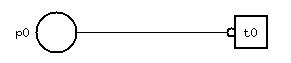
\includegraphics[height=12mm]{Arco_Inhibidor}}
  \subfigure[Arco Lector]{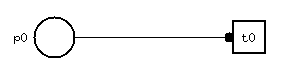
\includegraphics[height=13mm]{Arco_Lector}}
  \subfigure[Arco de Reset]{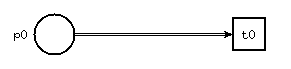
\includegraphics[height=13mm]{Arco_Reset}}
  \caption{Arcos Especiales}
  \label{fig:arcos_especiales}
\end{figure}

\subsection{Guardas}
\label{guardas}
% QUEREMOS EXTENDER EL MECANISMO DE SENSIBILIZADO
% POR AHORA LA SENSIBILIZACIÓN DEPENDE DEL ESTADO DE LA RED (MARCADO)

% ESTO PERMITE EXTENDER LA SENSIBILIZACIÓN DE FORMA NO AUTÓNOMA, PERMITE ASOCIAR
% LA SENSIBILIZACIÓN A UN ESTADO DEL MEDIO EXTERIOR
% LA GUARDA HACE UN AND CON LA FUNCIÓN DE SENSIBILIZACIÓN PARA DARLE MAYOR FLEXIBILIDAD
% LA GUARDA PUEDE SER POR TRUE O FALSE

Como se describió en la sección \ref{def_formal_petri}, una transición $t_{j}$
se encuentra sensibilizada si $$ \forall p_{i} \in \bullet t_{j}, m(p_i) \geq Pre(p_{i}, t_{j}) $$
Esto es, la sensibilización de $t_{j}$ depende únicamente del estado de
la red para un instante dado.

Si se pretende relacionar la RdP al estado del medio (estado de un sensor, del
programa que se ejecuta, etc), el modelo actual resulta no ser suficientemente
expresivo. Por esta razón, se introduce el concepto de \textit{guarda}.

Sea $V$ un conjunto de \textit{variables booleanas} con $v_{i} \in V$ y tal que
$\left\vert V \right\vert \leq \left\vert T \right\vert$

Si se asocia $v_{i}$ a $t_{j}$, se obtiene la guarda $g_{j}$ que puede tomar el
valor de $v_{i}$ o de su complemento $!v_{i}$ o $\mathtt{\sim} v_{i}$.

Cada variable $v_{i}$ afecta al sensibilizado de todas las transiciones que la
tengan asociada a través de cada guarda $g_{j}$, definiendo una nueva semántica
de sensibilización. Esta se resuelve realizando una operación AND entre el
estado de sensibilización de $t_{j}$ y el estado de su guarda asociada $g_{j}$.

A fin de formalizar este concepto, se construye un vector booleano $SG$ de
dimensión $t = \left\vert{T}\right\vert$, que se obtiene a partir de la
siguiente ecuación:

$$ SG = (V \times RP) \vee ( NV \times RN) \vee (NGT) $$
donde:
\begin{itemize}
  \item $NV \in B^{1 \times \left\vert V \right\vert} \slash  nv_{i} = \neg
  v_{i}$, el vector de variables $v_{i}$ negadas.
  \item $RP \in B^{\left\vert V \right\vert \times \left\vert T 
  \right\vert} \slash rp_{i,j} = True \Leftrightarrow g_{j} \in G \land g_{j} =
  v_{i} $, es decir que $t_{j}$ tiene asociada $g_{j}$ a $v_{i}$.
  \item $RN \in B^{\left\vert V \right\vert \times \left\vert T 
  \right\vert} \slash rp_{i,j} = True \Leftrightarrow g_{j} \in G \land g_{j} =
  \neg v_{i} $, es decir que $t_{j}$ tiene asociada $g_{j}$ a $!v_{i}$.
  \item $NGT \in B^{1 \times \left\vert T \right\vert} \slash ngt_{j} = True
  \Leftrightarrow g_{j} \not \in G$, es decir que $t_{j}$ no tiene guarda
  asociada.
  \item $\vee: B^{1 \times x} \rightarrow B^{1 \times x}$ es la
  función OR elemento a elemento (bitwise).
  \item $\times: B^{n \times m} \times B^{m \times p} \rightarrow B^{n \times
  p}$ es la función multiplicación de matrices booleanas.
\end{itemize}

De esta manera, $sg_{j}$ será $True$ si:
\begin{itemize}
  \item $t_{j}$ no tiene una guarda asociada
  \item El valor de la variable $v_{i}$ coincide con el de la guarda $g_{j}$
  asociada a $v_{i}$
\end{itemize}

Luego, si $f$ es la función de sensibilización utilizada hasta este punto, la
nueva función de sensibilización $f_{ext}$ es:
$$ f_{ext} = f \land SG $$

En la figura \ref{fig:guarda} se observa una plaza unida a una transición,
con una guarda asociada, referida a la variable \textit{\textbf{var}},
habilitada por $True$.

\begin{figure}[h]
  \centering
  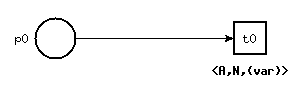
\includegraphics[height=15mm]{Guarda}
  \caption{Transición con guarda}
  \label{fig:guarda}
\end{figure}

\subsection{Semántica Temporal}

Muchos sistemas reales son dependientes del tiempo entre otras variables. Si
resulta de interés modelar un sistema de esta naturaleza, una RdP ordinaria no
es suficiente para hacerlo.

A raíz de esto es que se agrega comportamiento temporal a la semántica del
disparo de las Redes de Petri para obtener \textit{Redes de Petri Temporales}.

Entre las propuestas para agregar semántica temporal a las RdP, son del interés
de este proyecto integrador las Redes de Petri con semántica de \textit{Tiempo
Fuerte} y de \textit{Tiempo Débil}.

\subsubsection{Semántica de Tiempo Fuerte}

En sistemas del mundo real, las actividades no ocurren instantáneamente. Cada
actividad en un sistema tiene una duración distinta de cero, y se deberá asumir
que termina en un tiempo finito para poder modelarla.
\cite{Ramchandani:1974:AAC:889750}

En las RdP con semántica de tiempo fuerte, se asume que el disparo de una
transición toma un tiempo limitado, distinto de cero.

\begin{itemize}
  \stepcounter{definitionsCounter}
  \item [\underline{Definición \thedefinitionsCounter}:] Una Red de Petri Temporal con Semántica de
  Tiempo Fuerte es una tupla $(R, \Omega)$ donde:
  \begin{itemize}
    \item $R$ es una Red de Petri Ordinaria $R = \{P, T, F, W \}$
    \item $\Omega: T \rightarrow \mathbb{R^{+}}$ es una función que asigna
    a cada transición $t_{i} \in T$ un número real no negativo $\tau_{i}$,
    donde $\tau_{i}$ es el \textit{tiempo de disparo de} $t_{i}$
  \end{itemize}
\end{itemize}

\paragraph{Disparo de una Transición con Semántica de Tiempo Fuerte:}

Si $t_{i}$ es una transición que se encuentra sensibilizada, se la puede
disparar. Cuando se inicia el disparo, se retira la cantidad de tokens
correspondiente de $\bullet t_{i}$ y se dice que la transición $t_{i}$
\textit{se está ejecutando}.
La ejecución de $t_{i}$ dura un tiempo $\tau_{i}$, el tiempo de disparo de
$t_{i}$.
Cuando termina de transcurrir el tiempo $\tau_{i}$, se colocan los tokens
correspondientes en $t_{i} \bullet$ y se dice que el disparo \textit{ha
finalizado}.

No se permite comenzar el disparo de una transición que está ejecutando un
disparo anterior, es decir que por transición puede existir un único disparo en
ejecución.

Nótese que el disparo de una transición, pese a haber dejado de ser
instantánteo, sigue siendo atómico como en una RdP ordinaria.

\begin{figure}[h]
  \centering
  \subfigure[Antes]{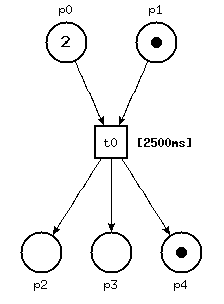
\includegraphics[height=45mm]{Tiempo_Fuerte_01}}
  \subfigure[Ejecución]{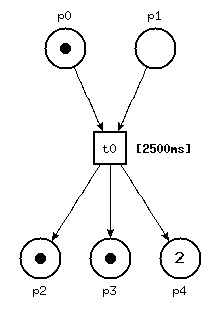
\includegraphics[height=45mm]{Tiempo_Fuerte_02}}
  \subfigure[Terminado]{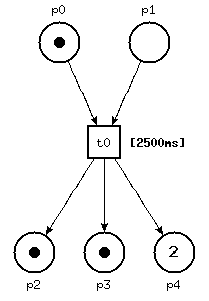
\includegraphics[height=45mm]{Tiempo_Fuerte_03}}
  \caption{Disparo de una transición con semántica de tiempo fuerte}
  \label{fig:disparo_tiempo_fuerte}
\end{figure}

En la figura \ref{fig:disparo_tiempo_fuerte} se observa una transición con
semántica de tiempo fuerte con tiempo de disparo de 2500ms en las tres fases del
disparo.

\subsubsection{Semántica de Tiempo Débil}

De forma más general que la Semántica de Tiempo Fuerte, la Semántica de
Tiempo Débil asigna a una transición $t$ un intervalo $[\alpha, \beta]$
denominado el \textit{intervalo de disparo} de $t$. Este intervalo puede ser cerrado o
abierto en cualquiera de sus extremos, y puede extenderse hasta el infinito. El
disparo de una transición sólo está permitido dentro de su intervalo de disparo.

Los tiempos $\alpha$ y $\beta$ son relativos al último instante de
sensibilización de $t$.
Esto es, si $t$ se sensibilizó por última vez en el instante $\theta$, el
disparo de $t$ sólo será posible en el intervalo $[\theta + \alpha, \theta
+ \beta]$. \cite{PetriNetsFundamentals}

\begin{itemize}
  \stepcounter{definitionsCounter}
  \item [\underline{Definición \thedefinitionsCounter}:] Una Red de Petri Temporal con Semántica de
  Tiempo Débil es una tupla $(R, IS)$ donde:
  \begin{itemize}
    \item $R$ es una Red de Petri Ordinaria $R = \{P, T, F, W \}$
    \item $IS: T \rightarrow \mathbb{Q^{+}} \times \{ \mathbb{Q^{+}} \cup \{
    \infty \} \}$ es la función de \textit{intervalo estático}.
  \end{itemize}
\end{itemize}

La función $IS$ asigna a cualquier transición $t \in T$ un intervalo con límites
racionales $IS(t) = [\alpha, \beta]$, con $0 \leq \alpha \leq \beta$. Solamente
$\beta$ puede adquirir un valor infinito.

El disparo de $t$ sólo está permitido en el intervalo de tiempo que tenga
relacionado. En el instante inicial (tiempo = 0), si $t$ está sensibilizada por
el marcado inicial, este intervalo coincide con el intervalo estático $IS(t)$.
Cuando el tiempo transcurre, el intervalo de $t$ avanza, corriéndose hacia el
origen una cantidad de tiempo igual al transcurrido desde el instante de
sensibilización. A este intervalo se le llama \textit{intervalo dinámico de disparo.}

Estos intervalos dinámicos pueden ser expresados como una aplicación $I$ que
asigna a cada transición $t$, un intervalo de tiempo $I(t)$ en el cual puede ser
disparada. Los límites del intervalo $I(t)$ son denominados el \textit{instante
menor de disparo} y el \textit{instante mayor de disparo}
correspondientemente. y son denotados $DMin(t)$ y
$DMax(t)$.\cite{PetriNetsFundamentals}

\paragraph{Estado de una Red de Petri Temporal:}

El estado de una RdP con Semántica de Tiempo Débil es un par $E = (M, I)$ donde
$M$ es el marcado de la red e $I$ es la \textit{aplicación de intervalos de
disparo}. El estado inicial $E_{0}$ consiste en la marca inicial $M_{0}$ y la
aplicación $I_{0}$ que asigna a cada transición sensibilizada su intervalo
estático y a las transiciones no sensibilizadas, el intervalo vacío.
Disparar una transición $t_{i}$ en el instante $\theta$ está permitido desde un
estado $E$, únicamente si se cumple:
\begin{itemize}
  \item La transición $t_{i}$ está sensibilizada por el marcado M.
  \item $\theta$ no es menor que el instante menor de disparo de $t_{i}$
  $$\theta \geq DMin(t_{i})$$
  \item $\theta$ no es mayor que el instante mayor de disparo de cualquier
  transición habilitada por $M$
  $$ \forall k, M \geq Pre(k) \Rightarrow \theta \leq DMax(k) $$
\end{itemize}

\paragraph{Disparo de una transición con Semántica de Tiempo Débil:}

El disparo de una transición $t_{i}$ en el instante $\theta$, desde el estado
$E = (M,I)$ lleva al estado $E' = (M', I')$ determinado de la siguiente manera:
\begin{itemize}
  \item El marcado $M'$ se determina igual que en una RdP Ordinaria.
  \item El intervalo $I'(t_{j})$ para cada transición $t_{j}$ se define:
  $$ I'(t_{i}) = \left\{
  \begin{array}{lll}
    \textnormal{Intervalo vacío} & si & t_{j} \textnormal{ no esta sensibilizada
    por } M \\
    IS(t_{j}) & si & t_{j} \textnormal{ entra en conflicto con } t_{i} \\
    \lbrack max(0, DMin(t_{j}) - \theta), DMax(t_{j}) - \theta \rbrack & si &
    t_{j} \textnormal{ está sensibilizada y } DMax(t_{j}) \in \mathbb{Q} \\
    \lbrack max(0, DMin(t_{j}) - \theta), \infty \rbrack & si & t_{j}
    \textnormal{ está sensibilizada y } DMax(t_{j}) = \infty \\
  \end{array}
\right.$$
\end{itemize}
Nótese que, a diferencia de la semántica de tiempo fuerte, el disparo de $t_{i}$
es instantáneo.

\begin{figure}[h]
  \centering
  \subfigure[Antes]{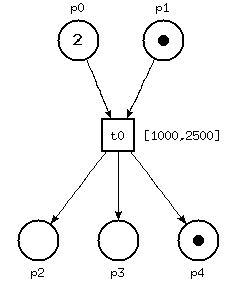
\includegraphics[height=45mm]{Tiempo_Debil_01}}
  \subfigure[Después]{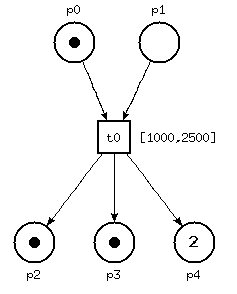
\includegraphics[height=45mm]{Tiempo_Debil_02}}
  \caption{Disparo de una transición con semántica de tiempo débil}
  \label{fig:disparo_tiempo_debil}
\end{figure}

En la figura \ref{fig:disparo_tiempo_debil} se observa el instante anterior y
posterior al disparo de una transición con semántica de tiempo débil. Para que
esto ocurra, el instante de disparo tiene que encontrarse dentro del intervalo
dinámico de disparo de $t_{0}$.

\begin{figure}[h]
  \centering
  \hspace*{\fill}
  \subcapcentertrue
  \subfigure[Transición con semántica de tiempo fuerte] {
    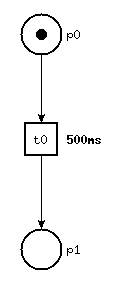
\includegraphics[align=c,height=50mm]{Tiempo_Fuerte_04}
    \label{fig:tiempo_debil_emula_fuerte_Fuerte}
  }
  \subfigure[Transición con semántica de tiempo fuerte modelada por transiciones
  con semántica de tiempo débil] {
    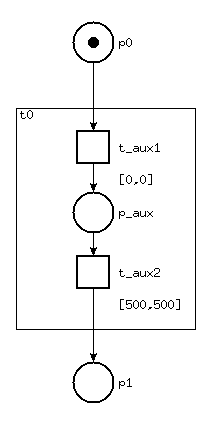
\includegraphics[align=c,height=75mm]{Tiempo_Debil_Emula_Fuerte}
    \label{fig:tiempo_debil_emula_fuerte_Debil}
  }
  \hspace*{\fill}
  \caption{Transición de tiempo fuerte modelada por tiempo débil}
  \label{fig:tiempo_debil_emula_fuerte}
\end{figure}

En la figura \ref{fig:tiempo_debil_emula_fuerte} se observa cómo, utilizando
transiciones temporales de semántica de tiempo débil, se puede modelar el
comportamiento de una transición de semántica de tiempo fuerte.
Para entender esta equivalencia, es conveniente repasar mediante un ejemplo el
disparo en ambos casos.

\subparagraph{Disparo en Tiempo Fuerte:}
Como se observa en la figura \ref{fig:tiempo_debil_emula_fuerte_Fuerte}, $t_{0}$ se
encuentra sensibilizada.
\begin{itemize}
  \item En el instante $\tau = 0$ se dispara $t_{0}$.
  \item Automáticamente se retira un token de $p_{0}$.
  \item Durante 500 milisegundos no ocurre nada.
  \item En $\tau = 500ms$ se coloca un token en $p_{1}$.
\end{itemize}

\subparagraph{Disparo en Tiempo Débil:}
Nuevamente, en la figura \ref{fig:tiempo_debil_emula_fuerte_Debil}, $t_{0}$ se
encuentra sensibilizada.
\begin{itemize}
  \item En el instante $\tau = 0$ se dispara $t_{aux1}$. Esto es posible ya que
  el intervalo de tiempo asociado lo permite.
  \item Se retira un token de $p_{0}$ y se coloca otro en $p_{aux}$.
  \item En ese instante se sensibiliza $t_{aux2}$ y se establece su intervalo dinámico.
  \item Durante 500 milisegundos no se puede disparar $t_{aux2}$.
  \item En $\tau = 500ms$ se dispara $t_{aux2}$, colocándo un token en $p_{1}$.
\end{itemize}

Así, visto desde el punto de vista de $p_{0}$ y $p_{1}$, en ambos casos el
comportamiento fue idéntico, con lo que se puede afirmar que la
semántica de tiempo débil tiene mayor expresividad y por lo tanto, es capaz de
modelar más situaciones del mundo real que la semántica de tiempo fuerte.


\subsection{Autonomía de una RdP}

Las redes de Petri analizadas en las secciones anteriores permiten modelar el
comportamiento de sistemas describiendo \textbf{qué} sucede en un proceso pero
no \textbf{cuándo} sucede.

Comunicando la RdP con el exterior del modelo, se puede controlar el momento (o
al menos el orden) con el que suceden los eventos. De esta manera, la RdP pasa a
ser \textit{no autónoma}.

\subsubsection{Red de Petri Autónoma}

En una RdP autónoma, se sabe que una transición puede ser disparada si está
sensibilizada, pero no se sabe cuándo o por qué será disparada.

Una extensión sobre este modelo son las \textit{\textbf{Redes de Petri
Estocásticas}}, donde a cada transición se le asigna una variable aleatoria
booleana $X$ con función de distribución de probabilidades $f$, que determina la
probabilidad de que se realice un disparo en un instante dado, si la marca $M$ lo permite.

Este tipo de modelos resulta súmamente útil para simular el comportamiento de
muchos sistemas del mundo real, ligados a variables aleatorias.

\subsubsection{Red de Petri No Autónoma}
En una RdP no autónoma, se asocia un evento $E^{i}$ a cada transición $t_{j}$ y
el disparo se da si $t_{j}$ está sensibilizada y $E^{i}$ ocurre.

Los \textit{eventos externos} corresponden a un cambio en el estado del medio
(incluyendo el tiempo). En cambio, un cambio del estado interno (del marcado),
se denomina \textit{evento interno}. La ocurrencia de un evento no tiene
duración. \cite{Hybrid_petri_nets}

\begin{itemize}
  \stepcounter{definitionsCounter}
  \item [\underline{Definición \thedefinitionsCounter}:] Una RdP sincronizada es una tupla
  $RdP_{Sync} = \{R, E, Sync\}$ tal que:
  \begin{itemize}
    \item $R =  \{P,T,F,W\}$ es una Red de Petri marcada.
    \item $E$ es un conjunto de eventos externos.
    \item $Sync : T \rightarrow (E \cup \{e\} ) $ donde $e$ es el evento
    que ocurre siempre.
  \end{itemize}
  \stepcounter{definitionsCounter}
  \item [\underline{Definición \thedefinitionsCounter}:] En una RdP no autónoma, una transición $t$
   es \textit{inmediata} o \textit{automática} si es disparada $q$ veces cuando
   está \textit{q-sensibilizada} $\forall q > 0$, a menos que existan conflictos
   entre dos o más transiciones.
\end{itemize}

Se dice que una transición sujeta a un evento externo es \textit{disparada}, de
otro modo será \textit{automática}. Esto se identifica en el modelo con una
etiqueta \textit{D} o \textit{F} para una transición disparada, y \textit{A}
para una automática.

\paragraph{Eventos estocásticos en redes de Petri no autónomas:}
Si una transición $t_{j}$ está sensibilizada, es disparada y espera la
ocurrencia del evento $E^{n}$ se disparará cuando $E^{n}$ ocurra.
Si a su vez se construye un generador de eventos $E^{n}$ sujeto a una variable
aleatoria $X$ con distribución de probabilidad $f$, se puede replicar la
semántica de una RdP estocástica utilizando una RdP no autónoma.
\footnote{Esta técnica se puede utilizar para depurar el modelo, agregando
eventos mediante simulación}

\subsection{Informes de Disparo}

De la misma forma que una RdP no autónoma permite actuar en función de eventos
provenientes del mundo exterior, los informes de disparo le brindan a la RdP la
posibilidad de emitir eventos hacia el medio. A su vez, estos eventos pueden
desencadenar acciones en observadores del mundo externo.

Una transición que emite eventos se denomina \textit{informada}.
Esto se denota con una etiqueta en la transición, indicando \textit{I} si es
informada, o \textit{N} si no lo es.

Para demostrar el potencial de este mecanismo, se analiza el siguiente ejemplo:

\begin{figure}[h]
  \centering
  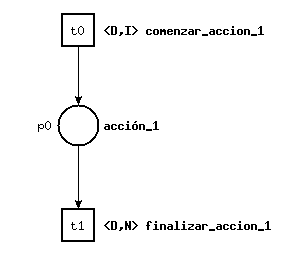
\includegraphics[height=50mm]{Emitir_Eventos_01}
  \caption{Emisión de Eventos ligados a acciones}
  \label{fig:eventos01}
\end{figure}

Si se relaciona una plaza $p_{0}$ con la ejecución de una
\textit{acción\textunderscore1} en el modelo, se puede aprovechar el mecanismo
de informes para sincronizar esta acción.

A continuación se describe una sucesión de eventos que aprovecha este
mecanismo, referido a la RdP de la figura \ref{fig:eventos01}:
\begin{itemize}
  \item Sucede un evento $E_{ext}^{0}$, $t_{0}$ lo escucha y de dispara.
  \item $t_{0}$ emite un evento $E_{int}^{0}$ avisando que fue disparada.
  \item Un observer de $E_{int}^{0}$ ejecuta \textit{acción\textunderscore1}.
  \item La finalización de \textit{acción\textunderscore1} emite un evento
  $E_{ext}^{1}$ hacia la RdP.
  \item $t_{1}$ escucha el evento $E_{ext}^{1}$ y se dispara.
\end{itemize}

\subsection{Política de Selección de Disparo}

Si existen múltiples transiciones sensibilizadas en una RdP, resulta de interés
tener un mecanismo de decisión que indique cuál debería ser la próxima
transición disparada.
Esta decisión resulta particularmente significativa en el caso de que dos o más
transiciones se encuentren en conflicto, ya sea un conflicto inmediato o un
conflicto que se genere luego de aplicar una sucesión de disparo $\sigma$.

El análisis del surgimiento de conflictos y de su posible resolución en redes de
Petri, lleva a algoritmos de búsqueda en árboles, con lo que su complejidad
crece exponencialmente con la profundidad del árbol a analizar, es decir, con
la cantidad de disparos futuros a analizar y con la cantidad de transiciones
analizadas. Esto lo hace imposible de aplicar para resolver problemas de
decisión de disparo por medio de la heurística.

La \textit{Política de Selección de Disparo} se refiere a la elección de la
próxima transición a disparar entre todas las sensibilizadas. Para una RdP,
incluidas la no autónomas o temporales, si esta elección es aleatoria el sistema
resulta no determinístico. Para que el sistema sea determinístico hay diferentes
soluciones, como la inclusión de: prioridades, probabilidades, arcos
inhibidores, arcos lectores. etc. \cite{Ecuacion_generalizada_LAC}

La política de selección de disparo $P : TS \rightarrow t \slash TS \subseteq T
\land t \in TS $ es una función que dado un vector de transiciones
sensibilizadas $TS$ indica cuál transición $t$ deberá ser disparada.

Para un determinado problema a resolver con una RdP, con conocimiento del
dominio del problema se puede diseñar una política de selección de disparos que
contemple los conflictos que puedan surgir, y priorice el disparo de
transiciones que generen situaciones más favorables para la solución de dicho
problema.

Cabe destacar que, pese a obtener un diseño correcto del modelo, una política
desfavorable al problema a tratar puede beneficiar ampliamente a parte de la
ejecución del modelo y perjudicar a otras, generando inanición sobre estas.


\section{Comparación entre Redes de Petri y Autómatas}
\label{comparacion_rdp_automatas}

Comparado a los autómatas, las RdP ofrecen una representación compacta de
sistemas concurrentes. Por esto, el modelado de este tipo de sistemas es
usualmente más natural usando redes de Petri. \cite{Iordache:2006:SCC:1197724}

Para comparar RdP y autómatas, se consideran sistemas compuestos por varios
subsistemas y se compara el tamaño de la RdP y el autómata que modelan el
sistema completo.

A fin de realizar esta comparación, es necesario previamente definir la
composición de autómatas y de redes de Petri.\cite{Iordache:2006:SCC:1197724}

\begin{itemize}
  \stepcounter{definitionsCounter}
  \item [\underline{Definición \thedefinitionsCounter}:] Sean $G_{1} = (Q_{1}, \Sigma_{1},
  \delta_{1}, s_{1}, F_{1})$ y $G_{2} = (Q_{2}, \Sigma_{2}, \delta_{2}, s_{2},
  F_{2})$ autómatas no determinísticos. La \textit{Composición Paralela} o
  \textit{Síncrona} de $G_{1}$ y $G_{2}$ es un autómata $G = G_{1} \parallel
  G_{2}$ que se define:
  $$ G = Ac(Q_{1} \times Q_{2}, \Sigma_{1} \cup \Sigma_{2}, \delta, (s_{1},
  s_{2}), F_{1} \times F_{2}) $$ donde $Ac$ es la función que elimina los estados no
 alcanzables de un autómata y $ \delta $ se define de la siguiente forma:
 \begin{itemize}
  \item [\underline{Definición \thedefinitionsCounter.1}:] Sea
   $$ \bar{\delta_{i}}(q,\alpha) =
   \left\{ 
     \begin{array}{lll}
      \delta_{i}(q, \alpha) & & \forall \alpha \in \Sigma_{i} \\
      \{q\} & & \forall \alpha \in (\Sigma_{1} \cup \Sigma_{2} \cup \{\lambda\})
      \backslash \Sigma_{i}
     \end{array}
   \right. $$
   para $i = 1,2$ y donde $\lambda$ es el evento nulo y $\backslash$ es la
   operación resta de conjuntos.
   Entonces: $$ \delta((q_{1},
   q_{2}), \alpha) = \bar{\delta_{1}}(q_{1}, \alpha) \times \bar{\delta_{2}}(q_{2}, \alpha) $$
 \end{itemize}
\end{itemize}

A fin simplificar el entendimiento de la composición de autómatas, se presenta
el siguiente ejemplo:

\begin{figure}[h]
  \centering
  \subfigure[$G_{1}$]{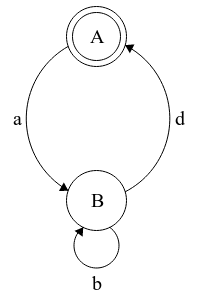
\includegraphics[height=45mm]{Composicion_Automata_1}}
  \subfigure[$G_{2}$]{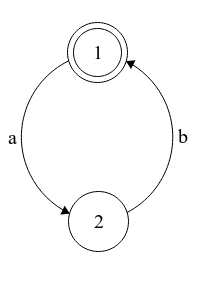
\includegraphics[height=45mm]{Composicion_Automata_2}}
  \subfigure[$G_{1} \parallel G_{2}$]{
    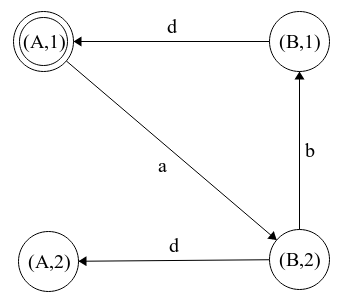
\includegraphics[height=45mm]{Composicion_Automata_3}
  }
  \caption{Composición de Autómatas}
  \label{fig:composicion_automatas}
\end{figure}

Sean $$G_{1} = (\{A, B\}, \{a, b, d\}, \delta_{1}, A, \{B\})$$ y $$G_{2} = (\{1,
2\}, \{a, b\}, \delta_{2}, 1, \{2\})$$ dos autómatas, entonces $G = G_{1}
\parallel G_{2}$ tendrá:
\begin{itemize}
  \item Estado inicial $(A, 1)$ ya que $A$ y $1$ son ambos estados iniciales.
  \item Estados finales $\{(B, 2)\}$ ya que $B$ y $2$ son estados finales.
  \item Las transiciones son:
  \begin{itemize}
    \item De $(A,1)$ a $(B,2)$ etiquetada con $a$ porque hay una transición de
    $A$ a $B$ y otra de $1$ a $2$, ambas etiquetadas con $a$.
    \item De $(B,2)$ a $(B,1)$ etiquetada con $b$ porque hay una transición de
    $B$ a $B$ y otra de $1$ a $2$, ambas etiquetadas con $b$.
    \item De $(B,1)$ a $(A,1)$ etiqueada con $d$, porque en $G_{1}$ hay una
    transición de $B$ a $A$ etiquetada con $d$, y como $d$ no existe en el
    conjunto de símbolos de $G_{2}$ no puede generar restricciones y según la
    definición genera una transición de $1$ hacia $1$.
    \item De $(B,2)$ a $(A,2)$ etiquetada con $d$ por la misma razón que la
    transición anterior. La transición de $A$ a $B$ existe en $G_{1}$, y se
    genera una de $2$ a $2$ en $G_{2}$
  \end{itemize}
\end{itemize}
    
\paragraph{Tamaño del autómata compuesto:}
Analizando el tamaño del modelo compuesto, asumiendo que todos los estados de
$Q_{1} \times Q_{2}$ son alcanzables desde el estado inicial, si $G_{1}$ tiene
$m_{1}$ estados y $G_{2}$ tiene $m_{2}$ estados, entonces $G_{1} \parallel
G_{2}$ tiene $m_{1} m_{2}$ estados. Es decir que la cantidad de estados de la
composición de autómatas es (o está acotada por) el \textbf{producto} de la
cantidad de estados de los autómatas que lo componen.

\begin{itemize}
  \stepcounter{definitionsCounter}
  \item [\underline{Definición \thedefinitionsCounter}:] Sean $R_{1} = (P_{1}, T_{1}, Pre_{1},
  Pos_{1}, \rho_{1})$ y $R_{2} = (P_{2}, T_{2}, Pre_{2}, Pos_{2}, \rho_{2})$
  redes de Petri etiquetadas donde:
  \begin{itemize}
    \item $\rho_{i} : T_{i} \rightarrow \Sigma_{i} \cup \{ \lambda \}$ para $i =
    1, 2$ es la función de etiquetado de las transiciones de $R_{i}$.
    \item $ \Sigma_{i} $ es el conjunto de símbolos del autómata equivalente a
    la i-ésima red de Petri
    \item $\lambda$ es el evento nulo
  \end{itemize} 
  La composición resulta en una red $R = (P, T, Pre, Pos, \rho)$ tal que $T$
  contiene las transiciones de $T_{1}$ y de $T_{2}$ que no están etiquetadas con
  $\lambda$ y las transiciones $t$ que modelan sincronizaciones de pares
  $(t^{1}, t^{2}) \in T_{1} \times T_{2}$ que comparten etiquetas distintas de
  $\lambda$.
  Se puede construir la red compuesta utilizando el siguiente algoritmo:
  \begin{enumerate}
    \item Sea $P = P_{1} \cup P_{2} $ y $T = \emptyset$.
    \item Sean $L_{1} = \bigcup_{t \in T_{1}} \rho_{2}(t) \backslash
    \{\lambda\}$ y $L_{2} = \bigcup_{t \in T_{2}} \rho_{1}(t) \backslash
    \{\lambda\}$.
    \item Para $i = 1, 2$, sea $T_{i,-} = \{ t \in T_{i}: \rho_{i} \backslash
    L_{i} \not = \emptyset \}$.
    \item Para $i = 1, 2, \forall t \in T_{i,-}$, sea $T = \{t\} \cup T$.
    $\rho(t) = \rho_{i}(t) \backslash L_{i}$. Sea $Pre(p, t) = Pre_{i}(p, t)$ y $Pos(p,
    t) = Post_{i}(p, t) \forall p \in P$ y sea $ Pre(p, t) = 0 $ y $ Pos(p,t) =
    0$ $\forall p \in P \backslash P_{i}$.
    \item Para cada par de transiciones $(t^{1}, t^{2}) \in T_{1} \times T_{2}$
    tal que $(\rho_{1}(t^{1}) \cap \rho_{2}(t^{2})) \backslash \{\lambda\} \not
    = \emptyset$, crear una nueva transición $t : T = {t} \cup T$, $\rho(t) =
    (\rho_{1}(t^{1}) \cap \rho_{2}(t^{2})) \backslash \{\lambda\}$ y hacer
    $Pre(p, t) = Pre_{i}(p,t)$ y $Pos(p, t) = Pos_{i}(p,t)$ $\forall p \in
    P_{i}$ para $i = 1, 2$.
  \end{enumerate}
\end{itemize}

Retomando el ejemplo de la composición de autómatas de la figura
\ref{fig:composicion_automatas}, se presenta la composición de las redes de
Petri equivalentes a dichos autómatas.

\begin{figure}[h]
  \centering
  \subfigure[$R_{1}$]{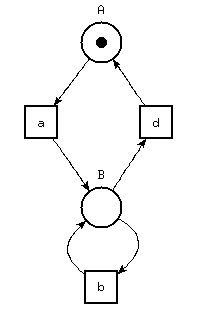
\includegraphics[width=35mm]{Composicion_Petri_1}}
  \subfigure[$R_{2}$]{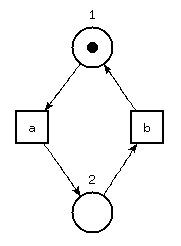
\includegraphics[width=30mm]{Composicion_Petri_2}}
  \subfigure[$R_{1} \parallel R_{2}$]{
    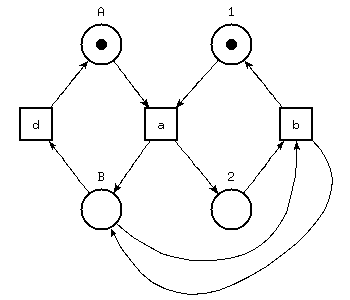
\includegraphics[width=65mm]{Composicion_Petri_3}
  }
  \caption{Composición de Redes de Petri}
  \label{fig:composicion_petri}
\end{figure}

\paragraph{Tamaño de la RdP compuesta:}
Si $R_{1}$ tiene $m_{1}$ plazas y $R_{2}$ tiene $m_{2}$ plazas, entonces $R =
R_{1} \parallel R_{2}$ tendrá $m_{1} + m_{2}$ plazas.
En contraste con el caso del autómata, la red de Petri compuesta crece
linealmente en cantidad de plazas respecto de las redes originales, es decir que
crece con la \textbf{suma} de las plazas de las redes originales.
Además, las transiciones de la red compuesta son las de las redes originales,
unificando las que comparten etiqueta. Es decir que la cantidad de transiciones
del modelo compuesto está acotada por la \textbf{suma} de las cantidades de los
modelos que lo componen.

\paragraph{Conclusión sobre la comparación de modelos:}
Analizando la forma en que crece el modelo resultado de	 la composición de
autómatas contra la composición de RdP se ve que estas últimás son más aptas para el modelado de
manera compacta de sistemas paralelos formados por subsistemas menores.
De la misma manera, una RdP permite modelar sistemas paralelos mucho mayores que
un autómata sin que el modelo resulte demasiado complejo para su análisis.
Otro punto a destacar es la existencia de un algoritmo para la composición de
redes de Petri, lo que permite la automatización de este proceso, simplificando
la tarea de construcción del modelo.
